\section{Results}
\label{sec:results}

\Cref{tab:results} lists every system on the development set. Cross-validation on the training data ranks the classical systems in the same order as the development set. Every development score is at or below its cross-validated mean, by 0.1 to 1.2 standard deviations and by 2.0 for n-grams alone, so the development set is somewhat harder than held-out training folds.

\begin{table*}[t]
\centering
\footnotesize
\setlength{\tabcolsep}{3.5pt}
\begin{tabular}{@{}lccccc@{}}
\toprule
System & Weighted F1 & Macro F1 & \SoftCons & \HardCons & CV weighted F1 \\
\midrule
Majority (\FW{} everywhere) & 0.129 & 0.112 & 0.000 & 0.000 & \\
Random, seed 13 & 0.246 & 0.240 & 0.184 & 0.054 & \\
\EQ{} everywhere & 0.110 & 0.104 & 1.000 & 0.314 & \\
\NO{} everywhere & 0.044 & 0.069 & 0.000 & 0.000 & \\
\midrule
Cues, logistic regression & 0.531 & 0.502 & 0.794 & 0.552 & 0.575 $\pm$ 0.037 \\
N-grams, logistic regression & 0.407 & 0.399 & 0.426 & 0.256 & 0.429 $\pm$ 0.011 \\
Cues and n-grams, logistic regression & 0.596 & 0.573 & 0.747 & 0.570 & 0.617 $\pm$ 0.021 \\
Cues, gradient-boosted trees & 0.574 & 0.550 & 0.718 & 0.527 & 0.572 $\pm$ 0.024 \\
\midrule
DeBERTa-v3-base, mean $\pm$ sd of 3 seeds & \textbf{0.807} $\pm$ 0.015 & \textbf{0.786} $\pm$ 0.017 & \textbf{0.877} $\pm$ 0.010 & \textbf{0.810} $\pm$ 0.013 & \\
\midrule
\textit{Pilot DeBERTa-v3-base, other track$^{\dagger}$} & \textit{0.75} & \textit{n/a} & \textit{0.84} & \textit{0.79} & \\
\bottomrule
\end{tabular}
\caption{Track 1 development set, official scorer. CV: cross-validation on the training data, five folds grouped by source pair, mean $\pm$ sd. For DeBERTa the held-out weighted F1 at the selected epoch averages 0.798. $^{\dagger}$Reported by \citet{apaolaza-larraya-etal-2026-assessing} on the PhrasIS positives track, without negatives and on another split; a reference point, not comparable.}
\label{tab:results}
\end{table*}

\paragraph{Surface cues buy consistency (H1).}
The cue-only model is the most self-consistent classical system: 220 of the 277 reversible pairs get compatible answers, and it confuses \FW{} with \BW{} in only 8 of the 380 directional instances. Its weights follow the EDA (\cref{tab:weights}): hypothesis-in-premise containment pushes towards \FW{} and away from \BW{}, its mirror does the reverse, and the length differences add a smaller push of the same kind. Because these cues swap or change sign under reversal, the model's decisions on a pair and its reversal are compatible almost by construction. Consistency is not correctness, though: 67 of its 220 consistent pairs are wrong in both directions, so \HardCons{} stays at 0.552.

\begin{table}[t]
\centering
\footnotesize
\setlength{\tabcolsep}{5pt}
\begin{tabular}{@{}lrrrr@{}}
\toprule
Cue & E & F & B & N \\
\midrule
$h$ words in $p$ & $-0.09$ & $+0.96$ & $-1.44$ & $+0.57$ \\
$p$ words in $h$ & $-0.02$ & $-1.35$ & $+0.97$ & $+0.41$ \\
Jaccard overlap & $-0.42$ & $+0.84$ & $+0.82$ & $-1.25$ \\
Character difference & $+0.01$ & $+0.49$ & $-0.49$ & $-0.01$ \\
Log word ratio & $-0.02$ & $+0.39$ & $-0.38$ & $+0.02$ \\
\bottomrule
\end{tabular}
\caption{The five largest standardised weights of the cue-only logistic regression, per label (E/F/B/N: \EQ, \FW, \BW, \NO).}
\label{tab:weights}
\end{table}

\paragraph{Inside the classical family, accuracy costs consistency (H3).}
Adding n-grams to the cues raises weighted F1 from 0.531 to 0.596 and lowers \SoftCons{} from 0.794 to 0.747; trees on the same cues show the same trade (0.574 and 0.718). The more expressive models find order-specific patterns that help single instances and break agreement across the pair. N-grams alone see the order only through bigrams that cross the separator, and score lowest on every metric.

\paragraph{The encoder gains on all three (H3 fails for it).}
DeBERTa-v3-base raises weighted F1 by 0.21 and \HardCons{} by 0.24 over the best classical system, and \SoftCons{} by 0.08 over the most consistent one (\cref{fig:tradeoff}). The gain is largest where the cues were weakest: against the combined classical model, F1 on \EQ{} rises from 0.45 to 0.78 and on \NO{} from 0.41 to 0.63, while the two directions rise from 0.72 and 0.71 to 0.86 and 0.87. Its consistency follows from correctness: only 16 to 21 of its consistent pairs per seed are wrong. We do not claim it beats the pilot, whose numbers come from another track, another split and a 150-trial search.

\begin{figure}[t]
\centering
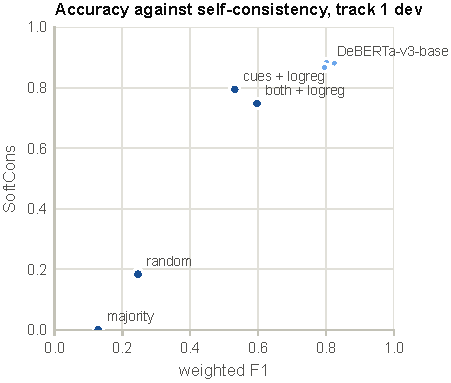
\includegraphics[width=\columnwidth]{figures/results-f1-vs-softcons}
\caption{Weighted F1 against \SoftCons{} on the development set; small points are the three DeBERTa seeds.}
\label{fig:tradeoff}
\end{figure}
